% !TeX root = ..\report.tex

\begin{figure}[ht]
    \centering
    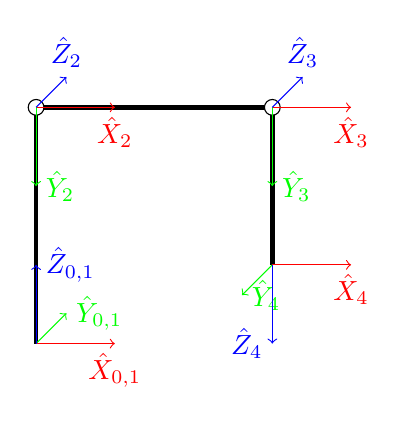
\begin{tikzpicture}
        % Arm 1
        \draw [ultra thick] (0, 0) -- (0, 3);

        \draw [->, red] (0,0,0) -- (1,0,0) node [below] {$\hat X_{0,1}$};
        \draw [->, green] (0,0,0) -- (0,0,-1) node [right] {$\hat Y_{0,1}$};
        \draw [->, blue] (0,0,0) -- (0,1,0) node [right] {$\hat Z_{0,1}$};

        % Arm 2
        \draw [ultra thick] (0, 3) -- (3, 3);
        \draw [fill=white] (0, 3) circle [radius=0.1];
        \draw [->, red] (0,3,0) -- (1,3,0) node [below] {$\hat X_2$};
        \draw [->, green] (0,3,0) -- (0,2,0) node [right] {$\hat Y_2$};
        \draw [->, blue] (0,3,0) -- (0,3,-1) node [above] {$\hat Z_2$};

        % Arm 3 and joint
        \draw [ultra thick] (3,3) -- (3,1);
        \draw [fill=white] (3,3) circle [radius=0.1];
        \draw [->, red] (3,3,0) -- (4,3,0) node [below] {$\hat X_3$};
        \draw [->, green] (3,3,0) -- (3,2,0) node [right] {$\hat Y_3$};
        \draw [->, blue] (3,3,0) -- (3,3,-1) node [above] {$\hat Z_3$};
        
        % Frame 4
        \draw [->, red] (3,1,0) -- (4,1,0) node [below] {$\hat X_4$};
        \draw [->, green] (3,1,0) -- (3,1,1) node[right] {$\hat Y_4$};
        \draw [->, blue] (3,1,0) -- (3,0,0) node[left] {$\hat Z_4$};
    \end{tikzpicture}
    \caption{固连坐标系分配}
    \label{fig:affixed-frame}
\end{figure}
